\documentclass[a4paper]{article}

\usepackage[T1]{fontenc}
\usepackage{lmodern}
\usepackage[utf8]{inputenc} 
\usepackage{graphicx}
\usepackage{wrapfig}

\title{Manual för QCornerGuardInspector}
\author{John Erlansson}
\date{2015-12-01}

\begin{document}

\pagenumbering{gobble}
\maketitle
\tableofcontents
\newpage

\pagenumbering{arabic}

\section{Användning}
	\subsection{Uppstart}
		När datorn startas skall programmet QCornerGuardInspector startas i
		helskärmläge.
		En genväg till programmet skall finnas på skrivbordet.

	\subsection{Åtgärder före uppstart}
		\subsubsection{Bländare}
			\begin{wrapfigure}{R}{6cm}
				\centering
				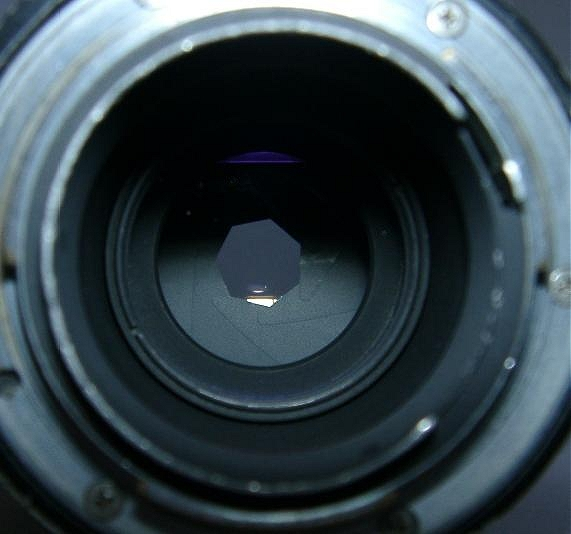
\includegraphics[width=4cm]{aperture.jpg}
				\caption{Bländare}
			\end{wrapfigure}
			Bländaren i en kamera är en anordning som reglerar mängden ljus som släpps in
			kamerahuset. Bländaren och slutartiden samarbetar för att exponera kamerans
			bildsensor, med rätt mängd ljus.
			
			Man kontrollerar att bilden har rätt mängd ljus genom att föra in en list i
			kameralådan så att en sträckkod är i bild. Bilden skall vara så ljus att
			sträckkoden inte flyter ihop, och så mörk att texten ändå har hög kontrast
			mot listen.

\subsubsection{Tröskelvärde}
		
	\subsection{Åtgärder under körning}
		\subsubsection{Återställning av larm}


\end{document}
